\documentclass[tikz,border=4pt]{standalone}
% Shared setup for the regression diagrams, in the AFRICAST palette
\usepackage{fontspec}
\usepackage[sfdefault,lining]{FiraSans}
\usepackage{amsmath}
\usepackage{unicode-math}
\setmathfont{Fira Math}
\usetikzlibrary{arrows.meta}
\definecolor{ink}{HTML}{1F2A36}
\definecolor{slate}{HTML}{434A5C}
\definecolor{AfricastBlue}{HTML}{3B75AC}
\definecolor{ochre}{HTML}{B5570F}
\definecolor{sageline}{HTML}{D9E2C8}
\definecolor{muted}{HTML}{6B7480}
\color{ink}
\tikzset{
  every picture/.style={>=stealth},
  every node/.style={font=\fontsize{9}{10}\selectfont},
  cell/.style={draw=sageline,fill=white,minimum width=#1,minimum height=.6cm,inner sep=0pt},
  cell/.default=1.2cm,
  head/.style={cell=#1,draw=slate,fill=slate,text=white,font=\fontsize{9}{10}\selectfont\bfseries},
  head/.default=1.2cm,
  on/.style={fill=AfricastBlue!15,text=AfricastBlue,font=\fontsize{9}{10}\selectfont\bfseries},
  base/.style={fill=ochre!12}
}

\begin{document}
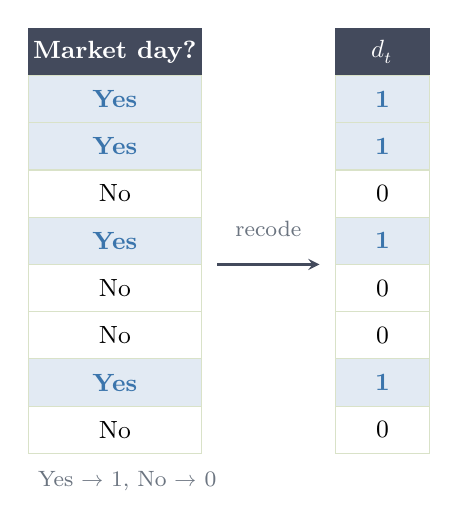
\begin{tikzpicture}
\node[head=2.2cm] at (0,0) {Market day?};
\node[head=1.2cm] at (3.4,0) {$d_t$};
\foreach \v [count=\i] in {1,1,0,1,0,0,1,0} {
  \ifnum\v=1
    \node[cell=2.2cm,on] at (0,-.6*\i) {Yes};
    \node[cell=1.2cm,on] at (3.4,-.6*\i) {1};
  \else
    \node[cell=2.2cm] at (0,-.6*\i) {No};
    \node[cell=1.2cm] at (3.4,-.6*\i) {0};
  \fi
}
\draw[->,thick,slate] (1.3,-2.7) -- (2.6,-2.7);
\node[font=\fontsize{8}{9}\selectfont,text=muted,align=center] at (1.95,-2.25) {recode};
\node[font=\fontsize{8}{9}\selectfont,text=muted,align=left,anchor=north west] at (-1.1,-5.2) {Yes $\to$ 1, No $\to$ 0};
\end{tikzpicture}
\end{document}
